\documentclass[11pt]{article}
\usepackage{graphicx}
\usepackage{cite}
\usepackage{xcolor}
\usepackage{listings}

\def\UrlBreaks{\do\/\do-}
\lstset{language=Fortran, 
  basicstyle=\small\ttfamily, 
  %identifierstyle=\color{green}, 
  numbers=left,
  commentstyle=\color{red}, 
  keywordstyle=\color{blue}, 
  showstringspaces=false 
}


\author{S.~V.~Adams, S.~Cusworth, C.~M.~Maynard and others}
\title{Report on LFRic computational performance 2019}
\date{\today}


\begin{document}
\maketitle
\medskip
\section{Introduction\label{sec:intro}}
The LFRic infrastructure is designed to host a dynamical core (Gung Ho)
that is scalable to a very large degree across a distributed memory
computer. This is typically expressed over MPI. LFRic is also designed
to accommodate different programming models to target different
processor architectures. Currently, OpenMP 2.0 is supported for shared
memory parallelism on CPUs. This is being extended to support OpenACC
to target both shared memory parallelism and Instruction Level
Parallelism (IPL) on GPUs. Moreover, the infrastructure has been
extended to support parallel, asynchronous I/O using the XIOS
client/server framework.
Other developments include the abstract solver API which allows for great
flexibility in constructing different solvers, redundant computation
algorithms into halo regions which boost the efficiency of shared
memory and reduce the amount of communication and finally a Multigrid
solver which will enable a large reduction in the cost of global communication.
Much of the model infrastructure is described in~\cite{LFRic}.

The LFRic model uses PSyclone to generate the Parallel System or PSy
layer. Here, data parallelism across the horizontal mesh is used,
exploiting both distributed and shared memory parallelism. This
exploits domain specific information, known to the science developer
and encoded as Metadata in the kernel layer. However, to
fully exploit the ILP on more parallel architectures such as GPUs, it
is necessary to extend PSyclone to fully parse individual Fortran
statements in the Kernel layer and then, for example, annotate the
source code with directives such as OpenACC or OpenMP. This work is just beginning,
however, the micro-benchmark~\cite{lfric-microbenchmarks} suite has been
developed so compute intensive kernels can be used to explore what kernel
optimisation can be developed which can then be generated by PSyclone in the full
model. The PSyclone Kernel Extractor (PSKE) is being developed to
allow the automated extraction of kernels, or more specifically a
driver with a dump file containing the necessary data for the looping
over the horizontal mesh and degrees of freedom without any of the
LFRic infrastructure.

LFRic uses Fortran 2003 Object Orientation programming to support many of the
features described above. This is a very powerful programming
style which aids software development by allowing a clear separation
of concerns between different areas of the code, promoting code re-use
and code development by disentangling dependencies. However, the lack
of compiler support, or more precisely, the proliferation of compiler
bugs which prevent the use of particular compilers, either without specific
code work arounds or even at all, is major problem. Development has
been severely delayed whilst compiler bugs have been isolated and
reported and work-arounds sought. The lack of working Fortran 2003
compilers remains a source of concern and must be considered a risk to
the project.

The strategy to obtain compute performance for LFRic has four main
strands. I/O performance is achieved by using the XIOS capability for
asynchronous parallel I/O in order to hide the cost of writing data.
Compute performance is achieved by enabling scalability, allowing
many agents to do computation. This comes at the cost of communication.
Local communication in the form of halo
exchange is reduced by employing a communication avoiding/reducing
algorithm of redundant computation into the halos and exploiting shared
memory threaded parallelism. Global communications are primarily in
the form of global sums required for iterative solvers. The global sum
is already vendor optimised both in the vendor supplied MPI library
implementation and the high-bandwidth, low-latency network of the
machine itself. The only way to reduce this cost and ultimate limit on
scalability is to use an algorithm with fewer global sums. This is the
Geometric multigrid pre-conditioner to the Helmholtz solver. The {\em
  on-node} compute performance of the LFRic code itself is examined by
considering the performance of computationally intensive kernels on
different processor architectures. The LFRic Microbenchmark suite can
be used to develop architecture specific optimisations.
The report is organised into sections on each of these four strands,
{\em viz.} I/O, local communication, global communication and
architecture specific optimisations.


\section{Independent section}
Code runs great etc.

\section{I/O}
The majority of the I/O infrastructure delivering diagnostic output in the form of UGRID-NetCDF via XIOS is on the LFRic trunk
and will be used as part of the Aquaplanet runs in 2019. Therefore it is now necessary to begin regular monitoring of the impact
of I/O on compute performance. In 2017, following the preliminary integration of XIOS into the LFRic infrastructure, performance
tests were done, focussing mainly on strong scaling of LFRic-XIOS for diagnostic output. The conclusion was that XIOS scaled well
out to 384 nodes (approx. 14K cores). A description of the work plus full results can be found in \cite{Adams2018}. 

For the 2019 report, the focus is on two main areas: strong scaling when outputting regular
diagnostics and also tests of in-situ post-processing. In particular tests have been done of time-meaning and also regridding 
from the LFRic native cubed-sphere mesh to a regular lat-lon mesh. Both of these are use cases from the upcoming Aquaplanet
runs and also evaluation of XIOS regridding is of interest to the wider Next Generation Modelling Systems programme as it
could inform how downstream processing will be handled. For instance whether LFRic can deliver Level 1 data directly to StaGE.
It could also make verification of LFRic easier if the data can be directly produced on a lat-lon mesh. The aim of the post-processing
experiments described here is primarily to get an idea of computational overhead in terms of runtime and memory, 
so there is no in depth analysis of scientific accuracy apart from verifying that the jobs have produced the right kind of output. 

\subsection{Job Setup}
All tests were performed on XCS. The executables were built from LFRic at r17102 using the LFRic Intel Fortran environment (17.0.0.098) 
including the latest PSyclone 1.7.0 and XIOS at r1537 of the XIOS trunk. Build flags were the default fast-debug which equates to:
-g -traceback -warn all -warn errors -ftrapuv -check all -fpe0 -O0 -stand f08

The science configuration was the standard baroclinic wave test with timestep length dependent on mesh resolution. 
For the purposes of the tests here: 900s for a C96 mesh and 180s for a C576 mesh.
10 fields are currently output as diagnostics in this configuration (air\_density (rho), three components of vorticity (xi1, xi2, xi3), eastward\_wind (u1), 
northward\_wind (u2), exner pressure (exner), divergence
of wind (divergence) on 30 half levels; air\_potential\_temperature (theta), upward\_air\_velocity (u3) on 31 full levels
which results in approximately 5 GB data per output

To keep within the PBS queue time limit the basic run is for 120 timesteps, with diagnostic\_frequency set to 20 timesteps.
This makes for 6 writes to a single UGRID-NetCDF file over the course of the run.

\subsection{Glossary of terms}

 
\begin{itemize}
  \item Client Ratio (CR).The percentage of time a client (model) task waits for the server. Ideally it should be as close to zero as possible.
  \item Client I/O time. The actual time (seconds) that the client task spends in I/O related activity
\end{itemize} 



\subsection{Set 1: Strong scaling}

This set of tests used a C576 mesh (approx 17Km horizontal resolution). Pure MPI only (\$OMP\_NUM\_THREADS=1). 
I/O setup used 12 XIOS servers with lustre stripe set count to be the same. This was the best performing setup from
the last set of I/O performance tests, so the assumption is that it is a good starting point.

\begin{table}[ht!]
\scriptsize
  \begin{center}
    \caption{Strong Scaling: Runtime}
    \label{tab:table1}
     \begin{tabular}{|c|c|c|c|c|c|}
      \textbf{Nodes} & \textbf{Max CR~(\%)} & \textbf{Max Client IO~(s)} & \textbf{Runtime no IO~(s)} & \textbf{Runtime~(s)} & \textbf{\% incr IO}\\
      \hline
      24 & 0.002 & 12.76 & 9832 & 10115 & +3\\
      54 & 0.002 & 13.30 & 4709 & 4950 & +5\\
      96 & 0.006 & 13.36 & 2810 & 2795 & -0.5\\
      216 & - & - & - & - & - \\
      384 & - & - & - & - & - \\
    \end{tabular}
  \end{center}
\end{table}

\begin{table}[ht!]
\scriptsize
  \begin{center}
    \caption{Strong Scaling: Memory Usage *}
    \label{tab:table2}
     \begin{tabular}{|c|c|c|c|}
      \textbf{Nodes} & \textbf{Memory Usage Gb (No IO)} & \textbf{Memory Usage Gb} & \textbf{\% incr IO} \\
      \hline
      24 & 764.3 & 841.3 & +10 \\
      54 & 936.8 & 1020.2 & +8 \\
      96 & 1126.4 & ? & ? \\
      216 & - & - & -  \\
      384 & -  & -  & -  \\
    \end{tabular}
  \end{center}
\end{table}

\scriptsize \textbf{* Note some job output does not include the PBS epilogue and so memory usage is not available (indicated by ?)}
\newline

\normalsize
The results are very similar to those done in the 2016/2017 tests (which were done with a C288 mesh). For the 24, 54 and 96 node jobs we see
evidence that scaling is preserved from the decreasing run times. The Client Ratio (CR) is very close to zero in all cases, 
showing that model client tasks are hardly waiting at all for I/O requests to be processed and that I/O is asynchronous.
The \% runtime penalty for I/O is low and well within the assumed machine variability. The \% memory usage penalty for I/O is approx 8-10\%. 

216 and 384 node jobs crashed out within the first few timesteps with XIOS-related errors even though no I/O was
actually happening at those timesteps. We assume that further tuning is needed for these higher node-count jobs.
See the Conclusions section for suggested avenues to explore.

\subsection{Set 2: In-situ Post-processing}

In this set of tests the focus is on regridding and simple time-meaning, with usage examples taken from latest Aquaplanet branch.
The aim here is to get an idea of computational overhead in terms of runtime and memory, and general correctness rather than scaling.
Therefore, these tests were done with a lower-resolution C96 mesh and only out to 96 nodes.
Runs have also been done to compare run time and memory usage to the same job configuration with only regular diagnostic output and also 
no I/O to get an idea of the additional penalty for using XIOS post-processing. 

\subsubsection{Averaging}

As Set 1, with the following changes: C96 mesh, 900s timestep.
In addition to regular diagnostics, averages are output over 20 timesteps, giving 6 writes to an additional file. 

\normalsize
\begin{figure}[ht!]
  \begin{center}
   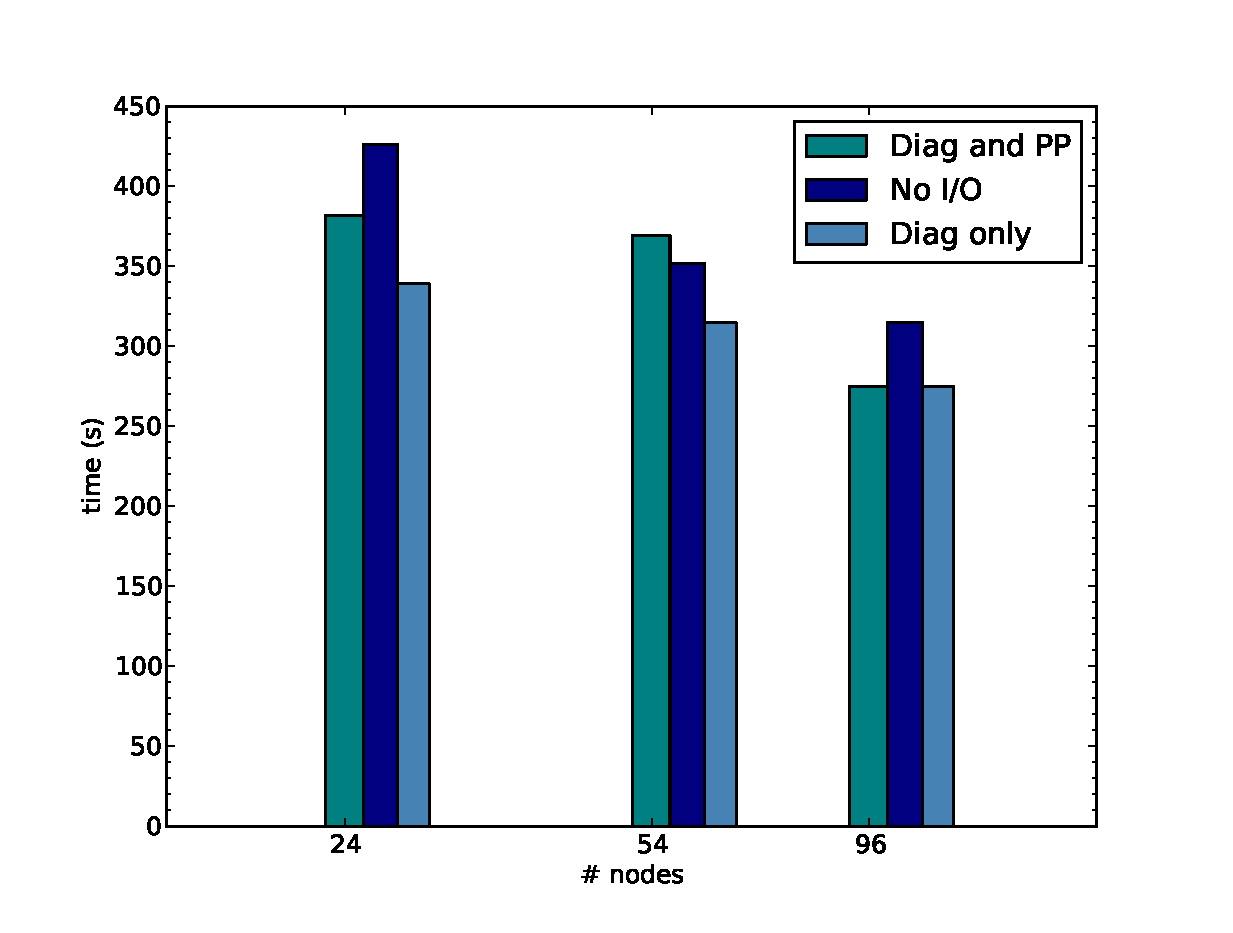
\includegraphics[scale=0.4]{figs/ave.eps}
   \caption{Averaging}
   \label{fig:fig1}
  \end{center}
\end{figure}

\begin{table}[ht!]
\scriptsize
  \begin{center}
    \caption{Averaging: Runtime}
    \label{tab:table3}
     \begin{tabular}{|c|c|c|c|c|c|}
      \textbf{Nodes} & \textbf{Max CR~(\%)} & \textbf{Max Client IO~(s)} & \textbf{Runtime~(s)} & \textbf{\% incr diag IO} & \textbf{\% incr no IO}\\
      \hline
      24 & 0.02 & 1.63 & 382 & -11 & +11 \\ 
      54 & 0.03 & 0.90 & 369 & +5 & +19 \\ 
      96 & 0.04 & 2.90 & 275 & -14 & 0 \\ 
    \end{tabular}
  \end{center}
\end{table}

\begin{table}[ht!]
\scriptsize
  \begin{center}
    \caption{Averaging: Memory Usage}
    \label{tab:table4}
     \begin{tabular}{|c|c|c|c|}
      \textbf{Nodes} & \textbf{Memory Usage Gb (pp) } & \textbf{Memory Usage Gb (diag only)} & \textbf{Memory Usage Gb (no IO)} \\
      \hline
      24 & 82.9 & 81.8 & 77.4 \\
      54 & 150.9 & 149.2 & 138.8 \\
      96 & 234.1 & ? & ? \\
    \end{tabular}
  \end{center}
\end{table}


Figure \ref{fig:fig1} gives a quick overview of scaling comparing run times for jobs without I/O, with regular diagnostic output and with
regular diagnostic output plus averaging. Scaling is still evident as run times generally decrease with the number of nodes. From
Table \ref{tab:table3}, the \% increases over just diagnostic output and no I/O are inconclusive - sometimes positive and sometimes negative. 
The range seems to be greater than for Set 1 so maybe a 5-10\% runtime penalty can be inferred, but it is difficult to say 
without doing runs to assess run time variability. Table \ref{tab:table4} shows a clear memory usage increase when adding different types of I/O. 
About +6-7\% for diagnostic I/O over runs with no I/O and a further +1\% for adding averaging post-processing. 


\subsubsection{Regridding}

As Set 1, with the following changes: C96 mesh, 900s timestep.
In addition to regular diagnostics, the rho, exner and divergence fields are regridded (to N96 equivalent) and output every 20 time steps, giving 6 writes to an additional file. Two sets of runs were done: computing weights on-the-fly each time and also using precomputed weights.

\normalsize
\begin{figure}[ht!]
  \begin{center}
   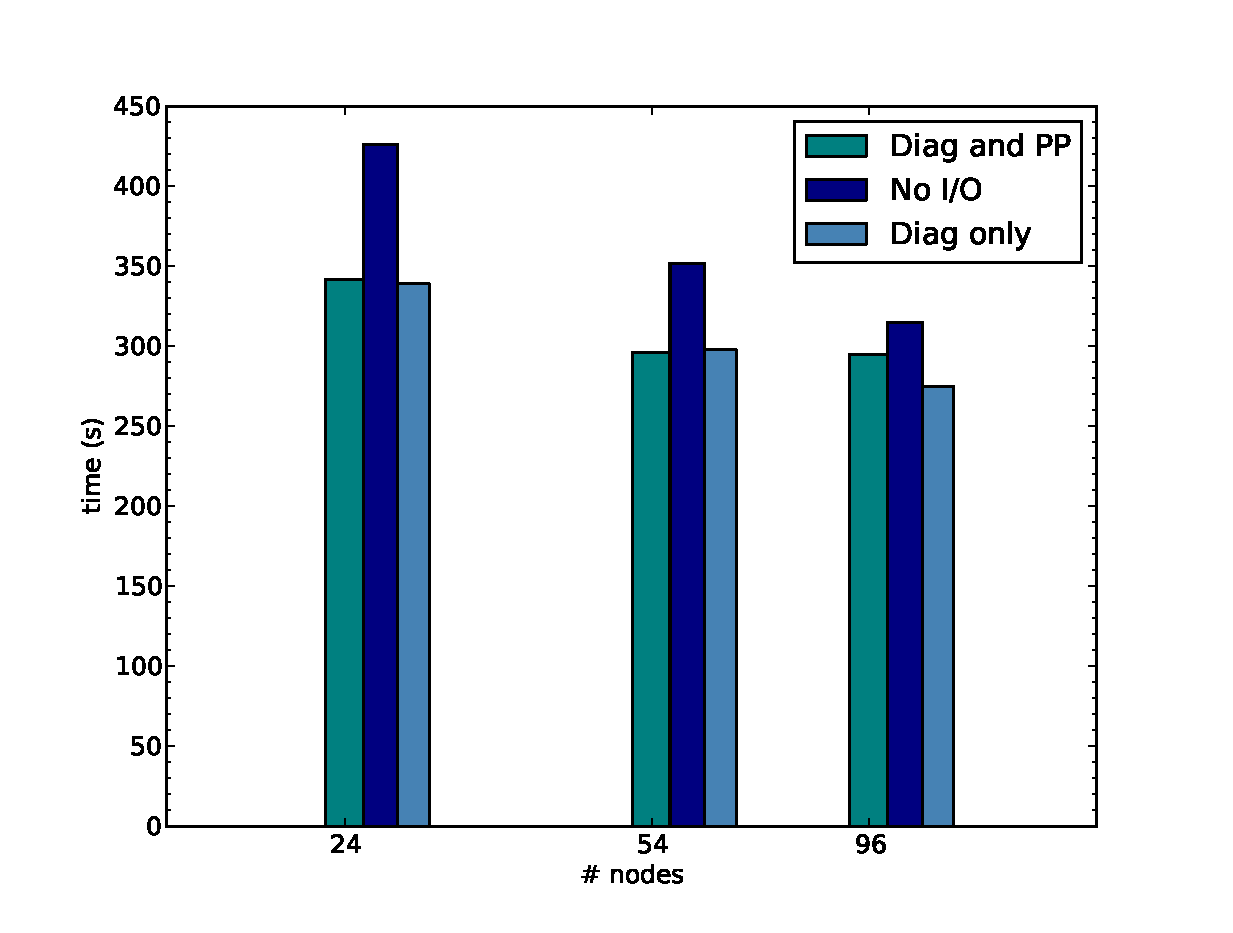
\includegraphics[scale=0.4]{figs/regrid.eps}
   \caption{Regridding (computing weights)}
   \label{fig:fig2}
  \end{center}
\end{figure}

\begin{figure}[ht!]
  \begin{center}
   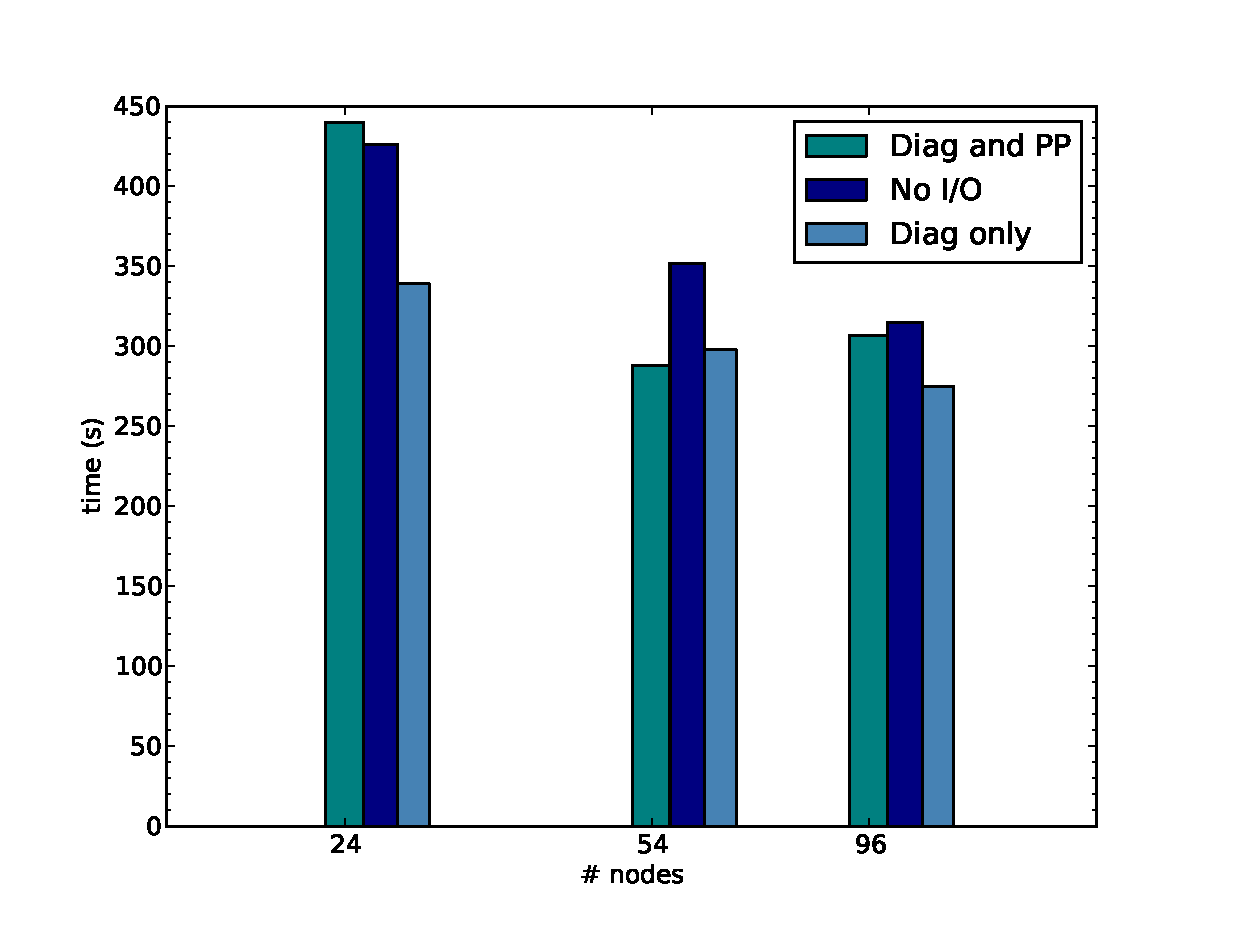
\includegraphics[scale=0.4]{figs/regrid_pcw.eps}
   \caption{Regridding (precomputed weights)}
   \label{fig:fig3}
  \end{center}
\end{figure}

\begin{table}[ht!]
\scriptsize
  \begin{center}
    \caption{Regrid, computing weights: Runtime}
    \label{tab:table5}
     \begin{tabular}{|c|c|c|c|c|c|}
      \textbf{Nodes} & \textbf{Max CR~(\%)} & \textbf{Max Client IO~(s)} & \textbf{Runtime~(s)} & \textbf{\% incr diag IO} & \textbf{\% incr no IO}\\
      \hline
      24 & 0.03 & 9.10 & 342 & -24 & +0.9 \\ 
      54 & 0.04 & 9.89 & 296 & -19 & -0.6 \\
      96 & 0.05 & 17.01 & 295 & -7 & +7 \\
    \end{tabular}
  \end{center}
\end{table}

\begin{table}[ht!]
\scriptsize
  \begin{center}
    \caption{Regrid, computing weights: Memory Usage}
    \label{tab:table6}
     \begin{tabular}{|c|c|c|c|}
      \textbf{Nodes} & \textbf{Memory Usage GB (pp) } & \textbf{Memory Usage GB (diag only)} & \textbf{Memory Usage GB (no IO)} \\
      \hline
      24 & 83.0 & 81.8 & 77.4 \\
      54 & 150.6 & 149.2 & 138.8 \\
      96 & ? & ? & ? \\
    \end{tabular}
  \end{center}
\end{table}

\begin{table}[ht!]
\scriptsize
  \begin{center}
    \caption{Regrid, precomputed weights: Runtime}
    \label{tab:table7}
     \begin{tabular}{|c|c|c|c|c|c|}
      \textbf{Nodes} & \textbf{Max CR~(\%)} & \textbf{Max Client IO~(s)} & \textbf{Runtime~(s)} & \textbf{\% incr diag IO} & \textbf{\% incr no IO}\\
      \hline
      24 & 0.02 & 7.07 & 440 & +3 & +30 \\
      54 & 0.04 & 3.30 & 288 & -18 & -3 \\
      96 & 0.04 & 4.32 & 307 & -3 & +12 \\
    \end{tabular}
  \end{center}
\end{table}

\begin{table}[ht!]
\scriptsize
  \begin{center}
    \caption{Regrid, precomputed weights: Memory Usage}
    \label{tab:table8}
     \begin{tabular}{|c|c|c|c|}
      \textbf{Nodes} & \textbf{Memory Usage Gb (pp) } & \textbf{Memory Usage Gb (diag only)} & \textbf{Memory Usage Gb (no IO)} \\
      \hline
      24 & 85.4 & 81.8 & 77.4 \\
      54 & 153.0 & 149.2 & 138.8 \\
      96 & 248.2 & ? & ? \\
    \end{tabular}
  \end{center}
\end{table}

\normalsize

From looking at the comparative runtimes in Figures \ref{fig:fig2} and \ref{fig:fig3} alone there is no clear benefit of computing weights each time vs using precomputed weights. As in previous results the general run time variability obscures things. Scaling is still evident as run times generally decrease with
increasing node count. Table \ref{tab:table7} gives a slight hint that client performance improves when using precomputed weights (lower CR and time spent in I/O).
Interestingly, memory usage increases slightly. Presumably there is a trade-off between the time and resources spent reading in the weights vs computing them.

\subsection{Conclusions}

Compared to the previous I/O performance assessment, in this year's tests the mesh resolution has been doubled and many more fields are output (although fewer timesteps are being run). A first assessment of the cost of in-situ post-processing has been made and is generally encouraging in that it seems to work correctly and there is no severe overhead of adding post-processing on top of regular diagnostic output. However, to get a really clear picture a thorough analysis of runtime variability for all non-I/O, diagnostic and post-processing scenarios is necessary. The post-processing tests need to be repeated with a higher resolution mesh as it may make any penalty more obvious (e.g. when computing regridding weights on the fly vs using precomputed weights). The issues seen with higher node count jobs need addressing to find out the cause. In the last I/O performance assessment no such problems were seen with 216 and 384 node jobs but many things have changed since then: the mesh is higher resolution and the LFRic dynamics and physics science schemes have changed considerably. 
We suggest several avenues of investigation:

\begin{itemize}
  \item XIOS buffer size. Normally not recommended to change this, but worth looking at as the error messages were to do with buffering and message passing
  \item Trying many more I/O servers
  \item Partial occupancy of nodes. If this is a memory problem then not fully occupying the nodes may help.
  \item Memory usage investigations to look at how memory usage changes during the run and what happens prior to a crash.
\end{itemize}


It is suspected that the issues are to do with memory usage and to
fully investigate this LFRic needs a way of regularly monitoring
per time-step memory usage as a matter of urgency.
 



\section{Optimisation for Processor Architectures
\label{sec:pa}}

\subsection{NVIDIA GPU}
The LFRic-microbenchmark suite~\cite{lfric-microbenchmarks} allows
optimisations for individual kernels to be explored without having to
compile and run the whole code. This is particularly useful when
targeting a programming model such as OpenACC for GPU architecture
where the Portland group compiler cannot compile the Fortran 2003 used 
in the main code.

The local matrix assembly (LMA) matrix-vector kernel had been
previously ported to run on GPUs by inserting Open ACC directives in
the PSy layer code to control the data transfer from host memory to
device memory and to offload the kernel call to the GPU device. This
Open ACC version was the starting point for Alan Gray from NVIDIA to
to look at optimisations. Moreover, after discussions regarding 
the PSyKAl API and the LFRic plans for how Open ACC will be
implemented for a GPU version, NVIDIA believe that the plan and
implementation will enable a succesful GPU implementation.
This is a summary of potential optimisations from NVIDIA.

\begin{lstlisting}[language=Fortran,caption={Code fragment of original 
    kernel},label={lst:LMA-orig}]
  !$acc loop vector 
  do k = 0, nlayers-1
    lhs_e(:,:) = 0.0_r_def
    ik = (cell-1)*nlayers + k + 1

    do df = 1, ndf1
      do df2 = 1, ndf2
        lhs_e(df,k) = lhs_e(df,k) + & 
          matrix(df,df2,ik)*x(map2(df2)+k)
      end do
    end do

    do df = 1, ndf1
      lhs(map1(df)+k) = lhs(map1(df)+k) + lhs_e(df,k)
    end do

  end do 
  !$
\end{lstlisting}

Shown in listing~\ref{lst:LMA-orig} is a code fragment of the LMA
kernel. It has an Open ACC directive \verb+!$acc loop vector+ before the
outmost $k$ loop, so that each thread in a thread block will do different loop
iterations. This code runs on a GPU, but not very efficiently. 

The first optimisation was to fuse the two loops over \verb+ndf1+
(lines 6-11 and 13-15) and replace the array \verb+lhs_e+ with a
scalar. The scalar can stay resident in a register for each thread and
avoids unnecessary memory accesses. This optimisation is call loop
fuse. 

The second optimisation was to exploit more parallelism on the GPU.
This performed with the Open ACC loop clause {\em collapse} to combine
the two outermost loops. This has the added benefit of aiding {\em
  memory coalescence}, {\em i.e.} neighbouring parallel threads
accessing neighbouring memory locations. However, an Open ACC {\em
  atomic update} directive is required as the loop over {\em ndf1} is
now also parallel. This optimisation is called Loop collapse. The new
kernel code is shown in listing~\ref{lst:LMA-opt}. 

\begin{lstlisting}[language=Fortran,caption={Optimised
    kernel},label={lst:LMA-opt}]
  !$acc loop vector collapse(2)
  do k = 0, nlayers-1
    do df = 1, ndf1

      ik = (cell-1)*nlayers + k + 1
      lhs_e_scal = 0.0_r_def

      do df2 = 1, ndf2
         lhs_e_scal = lhs_e_scal + & 
            matrix(df,df2,ik)*x(map2(df2)+k)
      end do
      
      !$acc atomic update
      lhs(map1(df)+k) = lhs(map1(df)+k) + lhs_e_scal

    end do
  end do
\end{lstlisting}

These first two optimisations increase the speed of execution but the
code still has a large register usage which results in low occupancy
of the GPU parallel units. This can be reduced by inlining the kernel
subroutine into the PSy layer. This can be done by the PGI compiler,
using Inter-procedural Analysis (IPA). This triggered by the following
compiler flag \verb+-Mipa=inline:reshape -Minfo flags+. The info flag
is for reporting purposes. This optimisation is called Inlining. 

The final optimisation is to note that the kernel is launched multiple
times, as the PSy layer includes the colouring ordering code for serialisation
to prevent race conditions. The kernel executes faster with a
single launch and NVIDIA optimised this by loop collapsing the loop
over colours and cells per colour. In the full code, this could be
simply done by not colouring at all. This optimisation is called
Single Kernel.

The colouring serialisation loop order is done for correctness,
however, the presence of the atomic update in the kernel prevents the
data race that colouring is designed to prevent, so the code is thread
safe. However, the atomic update doesn't guarantee the order of
execution, whereas colouring does. This means that whilst the data
race is avoided with the atomic update, the answer is not reproducible against
multiple runs. This is an optimisation which could be chosen for speed
when reproducibility is not an issue.

Shown in Table~\ref{tab:lma_nvidia} are the execution times for each
optimisation and in figure~\ref{fig:lma_nvidia} is shown the resulting
speed up versus the original code version.

\begin{table}
\centering
\caption{\label{tab:lma_nvidia} Execution times for different
  optimisations of a single run of  the LMA kernel on an V100 
  {\em Volta} NVIDIA GPU.}
\begin{tabular}{rc}
Optimisation & time (ms) \\\hline
Original     & $9.45$ \\
Loop fusion  & $5.33$ \\
Loop collapse & $2.68$ \\ 
Inlining      & $0.58$ \\
Single Kernel & $0.32$ \\\hline
\end{tabular}
\end{table}

\begin{figure}
\centering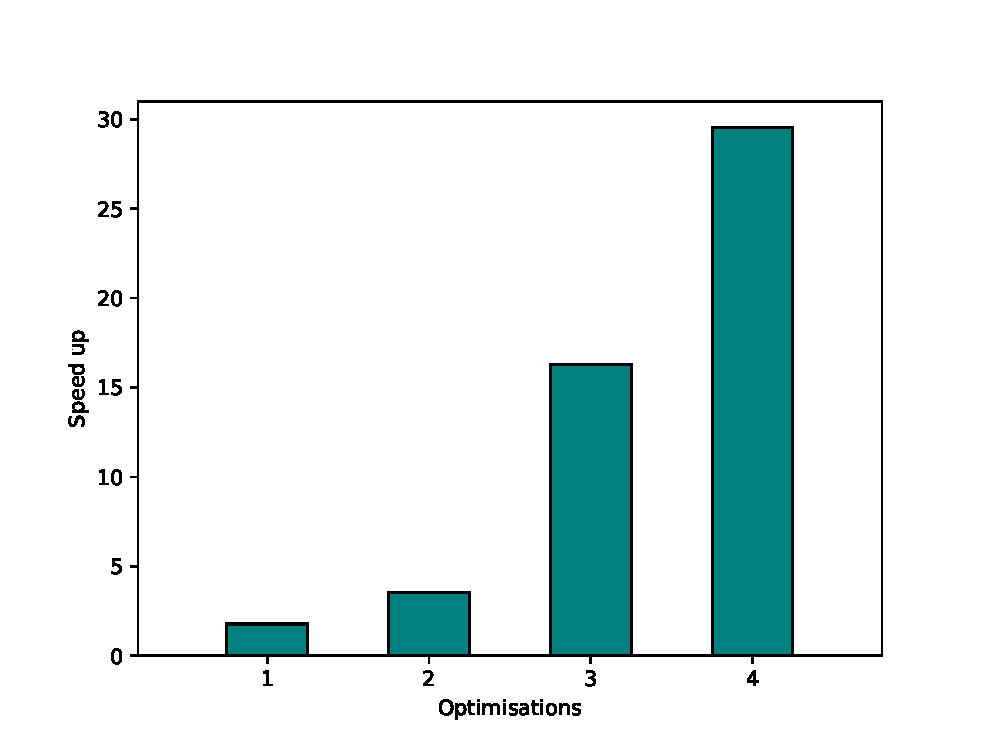
\includegraphics[width=1.0\linewidth]{figs/LMA-nvidia.eps}
\caption{\label{fig:lma_nvidia}Speed up of the LMA kernel against the
  original code for various optimisations. 1 loop fusion. 2 loop
  collapse. 3 Inlining. 4 Single Kernel.}
\end{figure} 

The speed up times are impressive, but a further analysis of the
absolute performance is useful. The NVIDIA profiler was
used to measure some performance metrics. This was compared to a simple ``roofline''
analysis~\cite{roofline} of the code on Volta. This suggests that as the arithmetic
intensity (flops per byte) of $0.3$ flops/byte of the kernel is low
compared to the ridge-line of the hardware, $9.9$ flops/byte, then the
code is memory bound. Comparing the memory bandwidth achieved of 549
GB/s to the Stream benchmark for the hardware suggests the code is
achieved around $70\%$ of the available bandwidth. This suggest the
code is fairly well optimised.

It should be noted that the problem size is too small, the data file
supplied to NVIDIA had $864$ cells with $40$ layers. Whilst, a target
local volume size of $12\times 12=144$ or $24\times 24=576$ is a
reasonable size for a single core of a CPU, a similar size is too
small to fully exploit the parallelism of GPU. In particular, to
effectively exploit the SIMT parallelism with the vertical degrees of
freedom, the vector size should be $128$ or more. $40$ levels is
clearly to few. Worse, in this particular case the colouring data here
had the non-optimal $6$ colours, whereas $4$ is sufficient. As seen in
the previous year's performance report the GPU should handle much more
work for a disproportional decrease in cost. This is especially true
for the number of levels.

These optimisations show that the code can run with some degree of
efficiency on a GPU. PSyclone is being developed so that is can
produce the necessary Open ACC directives in the PSy layer. Moreover,
its is being developed so that it can parse individual statements in
the kernel. This is necessary so that the kernel source can be
annotated with directives. Then the whole code can have a GPU
implementation generated automatically. To modify the actual source
code takes this a step further. However, it would in principle be
possible and moreover, this is similar to some of the ideas in CLAW~\cite{claw}.
CLAW is being considered for the parallelisation of the physical
parameterisations and some of the ideas would then be re-implemented in
PSyclone. Generating optimised code for GPUs is then possible.



\bibliography{refs.bib}
\bibliographystyle{unsrt}

\end{document}
